% vim: spelllang=en_au
\documentclass[a4paper]{article}

\usepackage{geometry}
\usepackage{amsmath}
\usepackage{enumerate}
\usepackage{amssymb}
\usepackage{amsthm}
\usepackage{hyperref}
\usepackage{minted}
% \usepackage[symbol]{footmisc}
\usepackage{tikz}
\usetikzlibrary{automata}
\usetikzlibrary{positioning,arrows.meta,calc}
\usetikzlibrary{angles,intersections,quotes,arrows.meta}


\DeclareMathOperator{\lcm}{lcm}

\author{Kait Lam \\ \small \texttt{45294583} \\ \small {T02}}
\title{\textsc{Math3306} --- Assignment 2 (Submission)}
\date{6 September 2024}

\begin{document}

\maketitle


\section*{Question 1}
\subsection*{Question 1(a)}
\begin{center}
  \textit{Must a language over a single-letter alphabet be regular?}
\end{center}
Of course not.
Even with only a single letter, it is sufficiently powerful to represent any set of natural numbers.
Define
\begin{align*}
  L = \{w \in \{\star\}^* ~|~ \ell(w) = \langle M, x \rangle \text{ and } \texttt{TM}_M\text{ halts on input }x\}.
\end{align*}
That is, the language of encoded pairs of Turing machine number and input, such that the Turing machine halts on the given
input.
This can be encoded as numerals in the usual way, i.e.\ by prime factors, then
this is further encoded as unary within our single-letter alphabet.
Were $L$ regular (that is, recognisable by a finite state automaton), this would easily decide the Halting problem,
contradicting the known undecidability of this problem.

Specifically, we could construct a TM which implements $\texttt{Halts}(m, x)$
by encoding $\langle m, x  \rangle$ into unary, then emulating the FSA of $L$ and returning 1/0 depending on whether the unary word is accepted/rejected.
As Turing machines are more powerful than FSA, this would be a straightforward task. 
(An FSA can also be translated directly into a TM,
e.g.\ like Q4(a) of Assignment 1).


% More generally, by way of encoding with prime factorisation and G\"odel numbering,
% any  can be represented as unary in a single-letter alphabet

% Assume, with the intent of contradiction, that $L$ is regular.
% It may be irregular.
% Consider the language
% \begin{align*}
%    L = \{ w \in \{\star\}^* ~|~ \ell(w)\text{ is prime}\}.
% \end{align*}
% Assume, with the intent of contradiction, that $L$ is regular and so the pumping lemma applies.
% By pumping, there exists $p_L > 1$ such that for all $w \in L$, 
% if $\ell(w) > p_L$, then there exists $x, y, z$ such that $w = xyz$ and 
% \begin{enumerate}[(i)]
%   \item $\ell(y) \ge 1$,
%   \item $\ell(xy)  < p_L$, and
%   \item $\forall n \ge 0, xy^nz \in L$.
% \end{enumerate}
% By property (iii), we can construct a word with non-prime length and assert it must be in $L$.
% To wit, the string
%   $xy^{2(\ell(x)+\ell(z))+1}z$.
% Observe,
% \begin{align*}
%   \ell(xy^{2(\ell(x)+\ell(z)+1)}z) &= \ell(x) + (2\ell(x) + 2\ell(z) + 1)\cdot \ell(y) + \ell(z) \\
%   &= 2(\ell(x) + \ell(z))\cdot(\ell(y) + 1)
% \end{align*}
% which is a non-prime length with factors $\ell(x) + \ell(z)$ and $\ell(y) + 1$.
% The pumping lemma claims this word is in $L$ which contradicts its original definition.
%
% As some technicalities,
% we note that due to infinitude of primes, we can obtain at least one $w \in L$ such that $\ell(w) > p_L$, in order to build our composite number.
% Also note that due to (i), $\ell(y) + 1 \ge 2$ and, due to (ii) and $\ell(xyz) > p_L$, $\ell(z) \ge 1$.
%
%
% x + n y + z
% x + 
% (2x + 2z) (y + 1) = 2xy + 2x + 2zy + 2z

% x + z + (2x + 2z) * y = x + z + 2xy + 2zy

\subsection*{Question 1(b)}
\begin{center}
  \textit{Recognise $L = \{0^{2n}~|~ n \ge 0\}$ with a Turing machine.}
\end{center}
We will write a recursive algorithm:
\begin{enumerate}[(1)]
  \setlength{\itemsep}{0pt}
  \item If the string is empty, accept.
  \item Otherwise, divide the input unary number by two in this way:
    \begin{enumerate}
      \item move right and clear every second space until the end of the string, then
      \item move left and compress the string, collapsing all cleared spaces.
    \end{enumerate}
  \item Go to (1).
\end{enumerate}
The division algorithm implicitly ensures that the number is divisible by two, otherwise it will halt
due to missing transitions.
The full Turing machine is shown in Figure~\ref{fig:tm}.
For easier reading, we use the single symbol 1 instead of 0.
Be assured that these are exactly equivalent.

\begin{figure}[h]
  \begin{center}
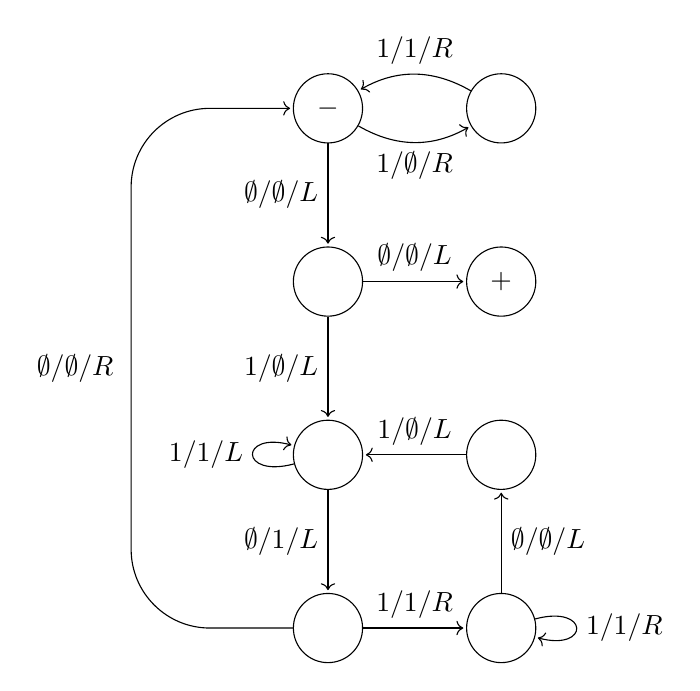
\begin{tikzpicture}[shorten >=1pt,node distance=2.2cm,on grid,auto] 

  \tikzset{
    rc/.style={rounded corners=2mm},
  }

   \node[state] (q0)   {$-$}; 
   \node[state] (first) [right=of q0] {};
   \path[->] (q0) edge [bend right] node [swap]{$1/\emptyset/R$} (first);
   % \node[state] (second) [right=of first] {};
   \path[->] (first) edge [bend right] node [swap]{$1/1/R$} (q0);

   \node[state] (base) [below=of q0] {};
   \path[->] (q0) edge node[swap] {$\emptyset/\emptyset/L$} (base);
   \node[state] (accept) [right=of base] {$+$};
   \path[->] (base) edge node {$\emptyset/\emptyset/L$} (accept);

   \node[state] (shift) [below=of base] {};
   \path[->] (base) edge node [swap]{$1/\emptyset/L$} (shift);
   \path[->] (shift) edge [loop left] node {$1/1/L$} (shift);

   \node[state] (shiftend) [below=of shift] {};
   \path[->] (shift) edge node [swap]{$\emptyset/1/L$} (shiftend);
   \node[state] (again) [right=of shiftend] {};
   \path[->] (shiftend) edge node {$1/1/R$} (again);
   \path[->] (again) edge [loop right] node {$1/1/R$} (again);
   \node[state] (restart) [above=of again] {};
   \path[->] (again) edge  node [swap]{$\emptyset/\emptyset/L$} (restart);
   \path[->] (restart) edge  node [swap]{$1/\emptyset/L$} (shift);

   \draw [->,rounded corners=1cm](shiftend) to
   ($(shiftend)+(-2.5, 0)$) to   node[xshift=-0.1cm]{$\emptyset/\emptyset/R$}($(q0)+(-2.5,0)$) to  (q0);
\end{tikzpicture}

  \end{center}
  \caption{A Turing machine.
     $\ominus$ and $\oplus$ denote the initial and accepting states, resp. 
  }\label{fig:tm}
\end{figure}

\section*{Question 2}
\begin{center}
  \textit{Is the language of (encoded) pairs of Turing machines with equivalent languages decidable?}
\end{center}
I think not.
If this language was decidable, it could be used to decide the halting problem.
We will demonstrate this.

Support $m$ and $x$ are given, encoding a Turing machine and an input under test.
We will compute $\texttt{Halts}(m, x)$.
First, transform $m$ into $m'$ such that
\begin{align*}
  T_{m'}(x') = \begin{cases}
    \textit{reject} &\text{if }x' \ne \text{$\star$}, \\
    \textit{accept} &\text{if }T_m(x)\text{ halts},\text{ and}\\
    \textit{undefined} & \text{otherwise}.
  \end{cases}
\end{align*}
Note that implementing $T_{m'}$ does \textit{not} require solving halting,
since we do not expect a concrete return value if $T_m(x)$ diverges.
$T_{m'}$ could be implemented from $T_m$ by %a simple check $x' = \text{``$\star$''}$, then
replacing all rejecting or missing edges
with an edge to an accepting state, 
then adding an initial check that $x' = \text{$\star$}$.
The language of $T_{m'}$ is $\{\text{$\star$}\}$ if $T_m(x)$
halts and $\emptyset$ otherwise.



% Note we use $T_m$ and $T_{m'}$ to refer to the TMs encoded
% by $m$ and $m'$, respectively.


Suppose, with suspicion, that we now have a decider for $\texttt{EQ}_{\text{TM}}$.
We could then run the 
$\texttt{EQ}_{\text{TM}}$
decider and ask whether
$T_{m'}$ has the same language as the Turing machine recognising precisely $\{\star\}$.
By decidability, we have that the decider \textit{will} return either \texttt 1 or \texttt 0
for all inputs,
and this will represent whether the given TMs have the same language.
To implement our
$\texttt{Halts}(m, x)$,
we simply propagate the result of the decider.

This decides the undecidable halting problem, a contradiction, and so $\texttt{EQ}_{\text{TM}}$
cannot be decidable.



% (arbitrarily) it takes its input as binary strings.
% We construct 
% \begin{align*}
%   \texttt{Halts}(m, x) &= \texttt{EQ}_{\text{TM}}()
% \end{align*}



\section*{Question 3}
\begin{center}
  \textit{Show the following predicate is primitive-recursive.}
\end{center}
Given $f$ and $g$ primitive-recursive,
\begin{align*}
  p(x) &= \begin{cases}
    1 & \text{if } f(i) > g(j),\text{ for all } 1 \le i \le x \text{ and } 1 \le j \le x,\text{ or } \\
    0 & \text{otherwise.}
  \end{cases}
\end{align*}
This can be expressed using bounded minimisation
(in this case, acting like bounded iteration).
\begin{align*}
  p(x) := \big(~x+1 = \mu(1\le i \le x).~(x+1 \ne \mu(1\le j \le x).~f(i) \le g(j))~\big)
\end{align*}
The desired predicate returns 1 iff $f(i)$ is always
greater-than $g(j)$ within
the square $1 \le i,j \le x$.
We implement this by searching within this region for counter-examples,
using bounded minimisation.
The bounded minimisation operator returns the least index satisfying its
argument function, if it exists, otherwise it returns one more than its upper bound.

We check the result of the inner $\mu$ to see if we have found \textit{any} counter-example,
and at the outer $\mu$, we check the inverse to ensure there have been \textit{no} counterexamples.
This will make sure we return the correct result of the predicate.
We assume the equality and disequality operators return either 0 or 1.

(Essentially, this encodes
\begin{align*}
  p(x) &= \neg \exists(1 \le i \le x).~\exists(1 \le j \le x).~f(i) \le g(j) \\
       &= \forall(1 \le i \le x).~\forall(1 \le j \le x).~f(i) > g(j),
\end{align*}
since $x + 1 \ne \mu(\cdot).~P$ implements $\exists(\cdot).~P$.)

\section*{Question 4}
\begin{center}
  \textit{
  Prove \textit{SOL} is NP-complete (both NP-hard and itself in NP).}
\end{center}

\end{document}

